\documentclass{article}
\usepackage[utf8]{inputenc}
\usepackage{amsmath,amsfonts,amssymb,amsthm,mathtools}
\usepackage{parskip}
\usepackage{color}
\usepackage{booktabs}
\usepackage{hyperref}

\newtheorem{exercise}{Exercise}
\newtheorem{answer}{Answer}

\newcommand{\dd}[2][]{\frac{\partial #1}{\partial #2}}
\newcommand{\dt}[2][]{\frac{d #1}{d #2}}
\newcommand{\dL}{\dt[{\L}]}
\newcommand{\dLi}{\dt[{\Li}]}
\newcommand{\dLmb}{\dt[{\Lmb}]}
\newcommand{\dLfb}{\dt[{\Lfb}]}
\newcommand{\yh}{\hat{y}}

\newcommand{\bracket}[3]{\left#1 #3 \right#2}
\newcommand{\sqb}{\bracket{[}{]}}
\newcommand{\ab}{\bracket{\langle}{\rangle}}
\renewcommand{\b}{\bracket{(}{)}}
\newcommand{\abs}{\bracket{\lvert}{\rvert}}

\newcommand{\0}{\mathbf{0}}
\newcommand{\x}{\mathbf{x}}
\newcommand{\y}{\mathbf{y}}
\newcommand{\f}{\mathbf{f}}
\newcommand{\h}{\mathbf{h}}
\newcommand{\g}{\mathbf{g}}
\newcommand{\mom}{\mathbf{v}}
\newcommand{\F}{\mathbf{F}}
\newcommand{\gfb}{\g_\text{fb}}
\newcommand{\gmb}{\g_\text{mb}}
\newcommand{\gmbt}{\g_{\text{mb}; t}}
\newcommand{\gsmbt}{g_{\text{mb}; t}}
\newcommand{\gsfb}{g_\text{fb}}
\newcommand{\gsmb}{g_\text{mb}}
\newcommand{\gsd}{\g_\text{sd}}
\newcommand{\vh}{\hat{v}}
\newcommand{\mh}{\hat{m}}
\newcommand{\gh}{\mathbf{\hat{g}}}
\newcommand{\gb}{\mathbf{\ab{g}}}
\newcommand{\gssqb}{\ab{g^2}}
\newcommand{\gsb}{\ab{g}}
\newcommand{\bv}{\mathbf{b}}
\newcommand{\ov}{\mathbf{o}}
\renewcommand{\a}{\mathbf{a}}
\newcommand{\X}{\mathbf{X}}
\newcommand{\W}{\mathbf{W}}
\newcommand{\I}{\mathbf{I}}
\renewcommand{\P}{\operatorname{P}\b}

\newcommand{\w}{\mathbf{w}}
\newcommand{\wo}{\w^*}

\renewcommand{\L}{\mathcal{L}}
\newcommand{\Lreg}{\L_\text{reg}}
\newcommand{\Lunreg}{\L_\text{unreg}}
\newcommand{\dLreg}{\dt[\Lreg]}
\newcommand{\dLunreg}{\dt[\Lunreg]}
\newcommand{\greg}{g_\text{reg}}
\newcommand{\gunreg}{g_\text{unreg}}
\newcommand{\Li}{\L_i}
\newcommand{\Lmb}{\L_\text{mb}}
\newcommand{\Lfb}{\L_\text{fb}}
\newcommand{\E}{\operatorname{E}\sqb}
\newcommand{\Var}{\operatorname{Var}\sqb}

\newcommand{\logits}{\ell}
\newcommand{\vlogits}{\boldsymbol{\logits}}
\newcommand{\softmax}{\operatorname{softmax}}
\newcommand{\linear}{\operatorname{linear}}
\newcommand{\relu}{\operatorname{relu}}
\newcommand{\sqerr}{\operatorname{sqerr}}

\newcommand{\func}{\operatorname{func}}
\newcommand{\funcback}{\operatorname{func{.}backward}}
\newcommand{\funcjac}{\operatorname{func{.}jacobian}}
\newcommand{\inputs}{\operatorname{inputs}}
\newcommand{\outputs}{\operatorname{outputs}}

\newcommand{\linearback}{\operatorname{linear{.}backward}}
\newcommand{\reluback}{\operatorname{relu{.}backward}}
\newcommand{\sqerrback}{\operatorname{sqerr{.}backward}}

\newcommand{\linearjac}{\operatorname{linear{.}jacobian}}
\newcommand{\relujac}{\operatorname{relu{.}jacobian}}

\newcommand{\iinmb}{{i \text{ in mb}}}
\newcommand{\mbsize}{M}
\newcommand{\mbavg}{\tfrac{1}{\mbsize} \sum_{\mathclap{\iinmb}}}

\newcommand{\iinfb}{{i \text{ in fb}}}
\newcommand{\fbsize}{N}
\newcommand{\fbavg}{\tfrac{1}{\fbsize} \sum_{i=1}^{\fbsize}}
\newcommand{\lrtrad}{\eta_\text{trad}}
\newcommand{\lravg}{\eta_\text{avg}}

\title{EMAT31530: Overfitting, and other topics in NN training}
\author{Laurence Aitchison}
\date{}

\begin{document}

\maketitle

I advise that you take a look at the iPython notebook for this week first, as it discusses overfitting in the simpler setting of linear models.  We take the next step, by discussing Here, we discuss overfitting in the more complex setting of neural networks and how to mitigate overfitting in these models.

\section{Overfitting is not catastrophic in NNs}

In the 1990's, neural networks were largely ignored: only a few people like Yann LeCun were still working on them.
One of the reasons was the following reasoning:
\begin{itemize}
  \item Neural networks have loads (and loads) of parameters.
  \item Models with loads of parameters tend to overfit.
  \item So neural networks should overfit really badly.
\end{itemize}
That led many people to expect that overfitting in NNs would be catastropic.
In actuality, it turns out that overfitting in NNs isn't catastropic at all: if you ignore overfitting while training your neural net, you should get a pretty reasonable fit.
But overfitting is still an issue, and there are a large number of approaches to mitigating overfitting in neural networks.
That's what we'll look at this week.


\newpage
\section{Weight decay}
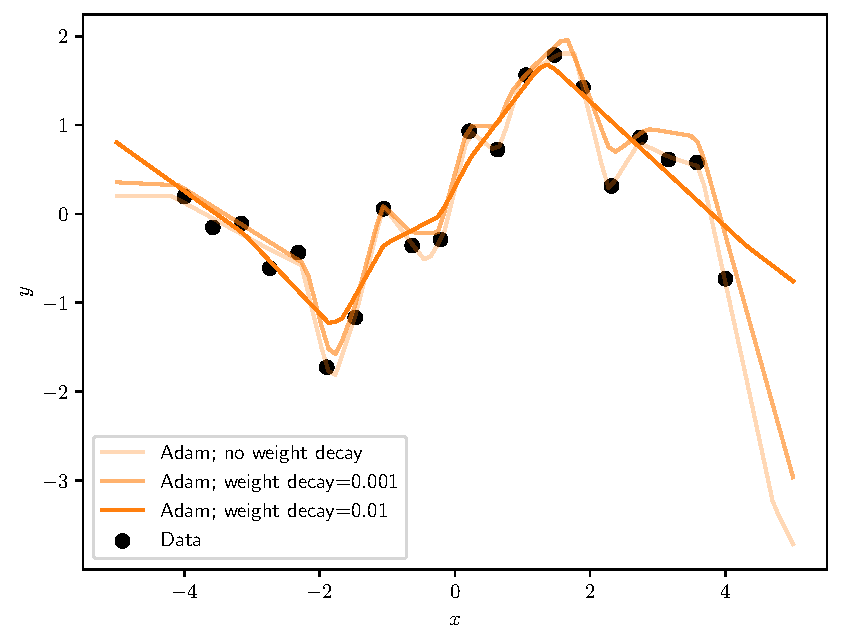
\includegraphics[width=\textwidth]{weight_decay.pdf}
Perhaps the most standard approach to mitigating overfitting is weight-decay.
In weight decay, we add a term to the loss, penalising large weights,
\begin{align}
  \label{eq:weight_decay_loss}
  \Lreg = \Lunreg + \tfrac{\lambda}{2} \sum_i w_i^2.
\end{align}
Here, $\Lunreg$ is the original unregularised loss (e.g.\ just the cross-entropy), and $\Lreg$ is the regularised loss.
To keep consistency with the \href{https://pytorch.org/docs/stable/generated/torch.optim.SGD.html}{PyTorch docs}, we assume that $\Lreg$ and $\Lunreg$ are either: 
\begin{itemize}
  \item the loss for a single minibatch.
  \item the \textit{average} loss across minibatches.
\end{itemize}
Importantly, this doesn't yet look like weight ``decay''.  

To understand where ``weight decay'' arises, consider the gradients for a single parameter, $w$,
\begin{align}
  \gunreg &= \dLunreg{w}\\
  \greg &= \dLreg{w} = \dLunreg{w} + \lambda w
\end{align}
Thus, the update becomes,
\begin{align}
  \Delta w &= \underbrace{- \eta \dLunreg{w}}_\text{original update} \underbrace{- \eta \lambda w}_\text{decay term}
\end{align}
Now, the $-\eta \lambda w$ is a decay term that pushes $w$ towards zero.

\newpage
\section{``Decoupled'' weight decay, or AdamW}
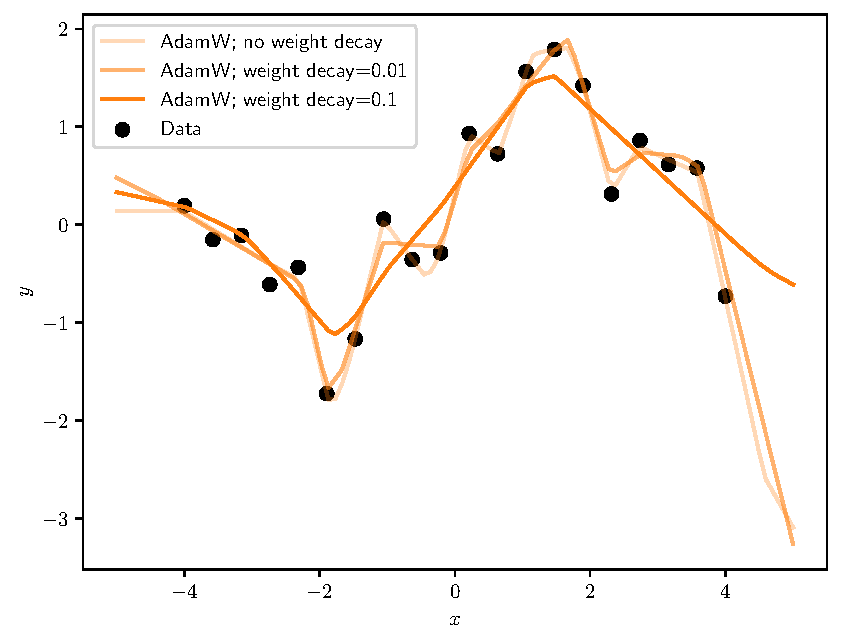
\includegraphics[width=\textwidth]{decoupled_weight_decay.pdf}
Almost all of deep learning is framed as optimization of loss functions.
That's why weight decay, which is fundamentally defined by Eq.~\eqref{eq:weight_decay_loss} makes alot of sense.
However, there is an alternative type of weight decay, which is these days used alot in training / finetuning transformers.
In particular, consider what happens with standard weight decay and Adam.
Remember that standard weight decay always works in terms of a modified loss.
So what happens when we put gradients of this modified loss into RMSProp?
\begin{align}
  \Delta w &= -\eta \frac{\greg}{\sqrt{\ab{\greg^2}}}\\
  \intertext{Substituting for the gradient of the regularised loss,}
  \Delta w &= -\eta \frac{\gunreg + \lambda w}{\sqrt{\ab{\greg^2}}}\\
  \intertext{And splitting up terms,}
  \Delta w &= \underbrace{-\eta \frac{\gunreg}{\sqrt{\ab{\greg^2}}}}_\text{original update} \quad\underbrace{- \eta \lambda \frac{w_i}{\sqrt{\ab{\greg^2}}}}_\text{Adam weight decay}
\end{align}
One thing you'll notive is that the updates no longer have a ``simple'' weight decay structure.  Instead, the weight decay is normalized by the squared gradient.
``Decoupled'' weight decay (or AdamW) is what you get when you remove the normalization (and you use the unregularised gradients in the denominator),
\begin{align}
  \Delta w &= \underbrace{-\eta \frac{\ab{\gunreg}}{\sqrt{\ab{\gunreg^2}}}}_\text{original update} \quad \underbrace{- \eta \lambda w_i}_\text{``decoupled'' weight decay}
\end{align}
This is \textit{super-weird} from the perspective of standard deep learning, as it can no longer be understood as gradient descent on a modified objective.
So why bother introducing AdamW?
Well, it seems to work well in particular cases like transformers, which is reason-enough for the deep learning community.

But we can go a bit further than that.
In particular, consider a single parameter, with a gradient, $g$, that's constant across minibatches and constant across a large range of parameters.
We can now solve for the steady-state value of $w$.
For Adam, as everything is framed in terms of an objective. 
Thus, we can find the steady-state by finding the location at which the gradients are zero,
\begin{align}
  0 &= \greg = g + \lambda w\\
  w &= -\frac{g}{\lambda}
\end{align}
So stronger gradients imply bigger weights.
In contrast, AdamW can't be framed in terms of an objective, so we need to work with the full updates,
\begin{align}
  \Delta w &= -\eta \frac{\ab{\gunreg}}{\sqrt{\ab{\gunreg^2}}} - \eta \lambda w_i.
\end{align}
Following the analysis of RMSProp last week, we're going to take,
\begin{align}
  \frac{\ab{\gunreg}}{\sqrt{\ab{\gunreg^2}}} \approx \text{sign}(\gunreg),
\end{align}
Thus, at steady-state,
\begin{align}
  0 &\approx -\eta \text{sign}(\gunreg) - \eta \lambda w_i,\\
  w_i &\approx \frac{\text{sign}(\gunreg)}{\lambda}.
\end{align}
So the steady-state weights for AdamW point in the same direction as the gradients, but they don't scale with the gradients!



\newpage
\section{Dropout}
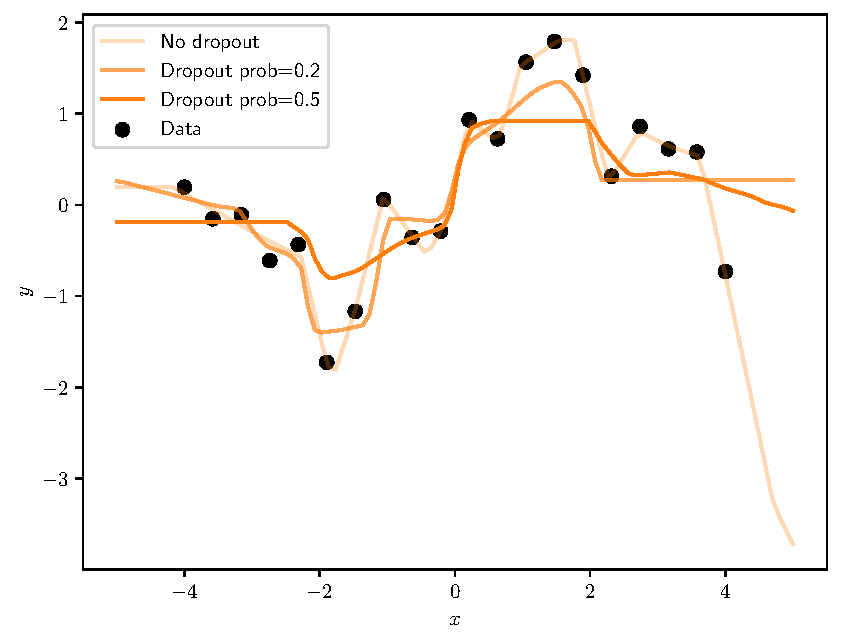
\includegraphics[width=\textwidth]{dropout.pdf}

\newpage
\section{Adam vs SGD}

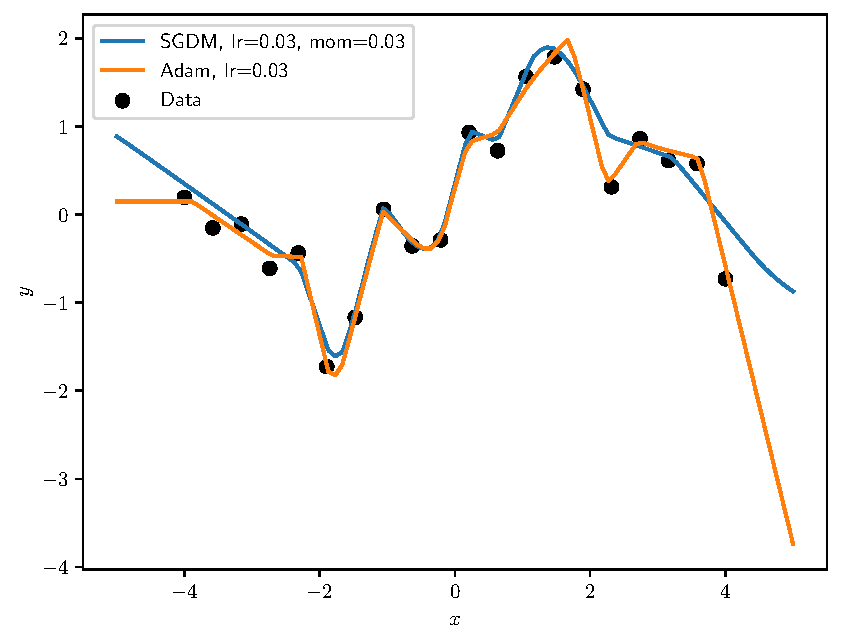
\includegraphics[width=\textwidth]{adam_vs_sgd.pdf}

Here, I ran both Adam and SGD for a long time (1000 iterations).
It seems that:
\begin{itemize}
  \item Adam is better at capturing ``fine details'' than SGD.
  \item Adam tends to overfit more than SGD.
\end{itemize}
Of course, these are really just two sides of the same coin: overfitting \textit{is} capturing the fine details (specifically, fine details in the noise).
Moreover, note that these patterns obviously depend on the ``hyperparameters'' (e.g.\ learning rate and momentum).  
But this is the general ``rule of thumb'' that does seem to hold very generally in NNs.

So which is best Adam or SGD?  Depends on whether you care about mitigating overfitting or capturing fine-details.
\begin{itemize}
  \item SGD tends to be better for ConvNets (which we'll look at next week) for image recognition, as it mitigates overfitting.
  \item Adam tends to be better for transformers (which we'll look at in a couple of weeks), RL where routing information in complex ways is important.
\end{itemize}

\newpage
\section{Early stopping}

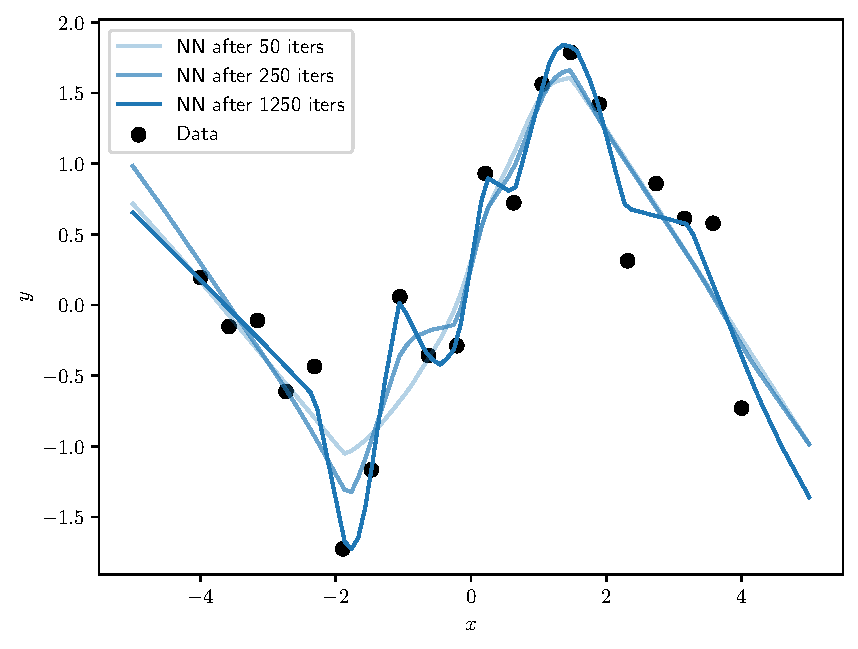
\includegraphics[width=\textwidth]{early_stopping.pdf}

Here, I fitted a three-layer network with width 100 hidden layer, to 20 datapoints drawn from $\sin(x) + \text{noise}$.
I used SGD with a learning rate of 0.01, and momentum of 0.8.
I then plotted the prediction at different points throughout training.

Late on in training (darker lines), the line basically goes through all the datapoints. Strictly speaking, this is overfitting, as its fitting the noise rather than the ``real underlying'' sin function (especially see the ``dip'' about $x=-1$.  
But this is still a pretty reasonable prediction, e.g.\ nothing has blown up.
Importantly, earlier in training (lighter lines) the function is smooth, it gradually gets more "details" as training progresses.
So we can use ``early stopping'' as a regularisation technique!
And early stopping is great because it gives us a nice excuse to cut training short (so training with early-stopping takes less time).

\newpage
\section{Minibatch noise}

\begin{center}
  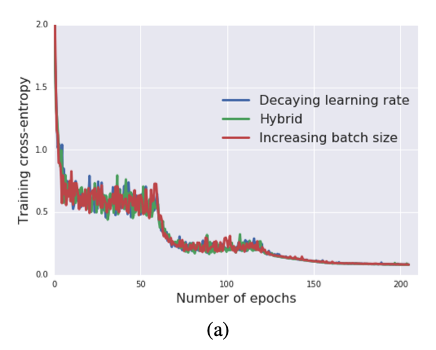
\includegraphics[width=0.5\textwidth]{schedule.png}
\end{center}

Typical practice in training neural networks involves starting with a high learning rate, then decaying the learning rate in steps.
In the above plot (blue line), the learning rate is decayed by a factor of 5 in steps at epochs 60 and 120 (epochs is a measure of time through training; one epoch means we've gone over all datapoints once).
Notice that as you decay the learning rate, the training cross-entropy drops quickly, then becomes somewhat static.
What seems to be going on is that minibatch noise stops you from converging to the actual optimum. to the real
Instead, minibatch noise causes you to bounce around the solution.
You can reduce the effective amount of noise by reducing the learning rate (see previous section on Optimizers).
Alternatively (red line), you can reduce the effective noise by increasing the batch size, so each batch averages over more datapoints.
However, we usually reduce the learning rate rather than increasing the batch size, as we don't have the GPU memory to increase the batch size.


\newpage
\section{High learning rates}

\begin{center}
  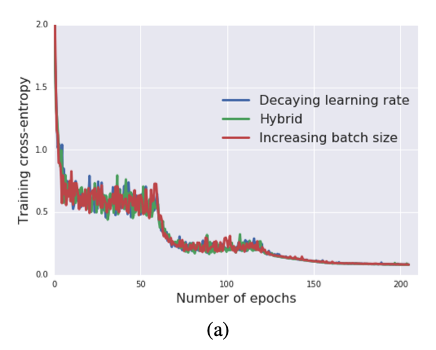
\includegraphics[width=0.5\textwidth]{schedule.png}
\end{center}

The previous plot would suggest that we should aggressively reduce learning rates.
But that isn't true!
Specifically, loss landscapes look


\section{Exercises}

\begin{exercise}
\end{exercise}

\begin{answer}
\end{answer}


\end{document}

